\title[PRIVO\@: securely and PRIVately Verificable PROtests]{%
  PR$^{^{\text{I}}\text{V}^{\text{ately}}_\text{erifiable}}_{\text{Otests}}$%
  %PRIVO\@:
  %SPRIVO\@:
  %Securely and Privately Verifying Protests
  %securely and PRIvately Verifiable PROtests
  %Verifying Protests
  %Verifying Demonstrations
  %Verifying Real-World Protests
  %Verifying Physical Protests
  \thanks{%
    An initial discussion of this work appeared in 
    \citetitle{FutureProtests}~\cite{FutureProtests}.
  }
}

\maketitle

\mode*

\begin{abstract}
  \begin{abstract}
% What's the problem?
The problem of participation estimation is a fundamental democratic issue in the context of physical protests or demonstrations.  There, the number of participants reflects the strength of the support or at least interest of the public society towards the topic of the protest.
%Seb: I put this part in comment because I think it is better to keep the scenario for the introduction and rather to be short in the abstract
%We consider the following scenario. Alice organizes a protest against the current regime leader Grace.
%The protest is held in some location(s) and Alice wants to estimate 
%the number of participants to prove a certain support for her cause.
% Why is it a problem?
Current methods for crowd counting have wide margins for error in addition to being generally quite privacy-invasive.
Moreover, the organizers of the protest may be tempted to cheat by inflating the number of participants as much as possible whereas it is in the government's interest to do the opposite if the protest is directed against it.                                                                                  
% What's the approach?
In this paper, we propose a novel approach to this problem by combining location proofs with some properties of electronic voting to provide verifiable yet privacy-preserving participation counts.
Since the parties have incentives to cheat, transparency is a fundamental requirement that we achieve through a decentralized scheme providing both verifiability and privacy.
More specifically, the proposed scheme is distributed, does not depend on any authority and it must scale to handle large protests (\ie millions of participants).
%
In our scheme, each participant creates a participation proof with the collaboration of other participants, called witnesses, in a privacy-preserving manner (\ie without requiring to reveal their own identity or that of witnesses).
The blockchain is used to commit and timestamp the participation proofs, which essentially consist of location proofs in which a privacy-preserving distance-bounding protocol is used by a participant to prove their proximity to the witnesses.
% What's the result?
Our scheme provides verifiability, which means that each participant can verify that their participation has been included in the final count--- \ie individual verifiability, 
to prevent the regime in place from dropping data --- and that anyone can verify the correctness of the result --- \ie universal and eligibility verifiability, to prevent any malicious actor (\eg Sybil attack) from affecting the result. \sonja{more scientific results?'}
%Seb: we need to be careful about how we formulate the following sentence
%Our scheme provides these verifiability properties in a privacy-preserving manner in the sense that it adds no risk to a participant that was not already present when not using our scheme. 
\end{abstract}

%\keywords{%
%  Crowd estimation;
%  Protest;
%  Electronic voting;
%  Location proof;
%  Distance-bounding;
%  Privacy.
%}
%

\end{abstract}

\clearpage
\tableofcontents
\clearpage

% What's the problem?
% Why is it a problem?
% What's the approach?
% What are the results?
\mode<all>{%
\section{Introduction}%
\label{Introduction}

Consider the following scenario in which Alice is an activist that organizes a protest against the current regime leader Eve in some location(s).
On one hand, Alice wants to estimate the number of participants to prove a certain support for her cause.
On the other hand, Eve is an autocrat who opposes Alice's cause.
Bob, Carol and many others participate in the protest for Alice's cause against Eve.
However, they might also be willing to do so in a manner that does not leave any digital traces because of the fear of retribution against them from Eve's regime. 
To verify how many participated in Alice's protest, a reliable yet privacy-preserving crowd-counting mechanism is needed, which to the best of our knowledge is a problem that has not yet been entirely solved.

After many demonstrations the count by police and that by the organizers 
differ, for legitimate\footnote{%
  A difference is actually quite natural, as the counts have different goals.
  The organizers want to count everyone who ever participated.
  Police want to estimate the count at the peak of participation, due to crowd 
  control~\cite{2016DemonstrationsInSeoul}.
} or other reasons, in some instances the difference can be hundreds of thousands.
There are numerous examples where there is difficulty in establishing the actual 
number of participants, e.g.:\@ the demonstrations against the president in 
South Korea~\cite{2016DemonstrationsInSeoul}, Trump's inauguration 
attendance~\cite{HowWillWeKnowTrumpInauguralCrowdSize}, the 2017 Women's March 
in the US~\cite{2017WomensMarchesInUS}, the demonstrations against changing the 
constitution in Venezuela~\cite{AlJazeeraOnVenezuela2017} or for the 
independence of Catalonia~\cite{CataloniaDemonstrations}.
The methods for counting the crowds vary.
Most of the available methods lack precision, i.e.\ they have large error 
margins.
They can only give an estimate for a particular snapshot in time, e.g.\ at the 
peak of the event, not the cumulative participation count --- at least not 
without counting some people multiple times, which in turn increases the error 
of the estimation.
Finally, they also lack verifiability, i.e.\ everyone must trust the entity who
does the counting.
(We will discuss them in more detail in \cref{RelatedWork}.)

We can make one important observation about this problem that has not
been adequately addressed in the design of existing crowd-counting solutions: it is an adversarial setting.
Alice the activist has an incentive to increase the tallied number of 
participants, whereas Eve (and possibly other interests) have an incentive to 
decrease the tallied number of participants.
In this case we have two options:
either we trust Alice or Eve, or we must verify their claims.
Our main goal is to provide a scheme which prevents both Alice and Eve from 
cheating, i.e.\ we aim for verifiable claims.
To solve this problem, we need a verifiable participation count which is 
protected from Sybil attacks while still preserving the participants'
privacy to the extent possible given their physical presence at the protest.

\subsection{Combining properties of electronic voting with location proofs}

In general, protesting is very similar to petitions, which in turn are similar 
to voting: all three are many individuals expressing their opinion.
These opinions can be sensitive, e.g.\ cause for discrimination or persecution, 
hence we desire to have similar properties of verification and privacy for 
verifying a protest as there is for voting.

Voting has (generally) three desirable requirements for 
verifiability~\cite{VerifyingPrivacyPropertiesOfVotingProtocols}.
\begin{description}
  \item[Eligibility] anyone can verify that each vote cast is legitimate.
  \item[Universal verifiability] anyone can verify that the result is according 
    to the cast votes.
  \item[Individual verifiability] every voter can verify that their vote is 
    included in the result.
\end{description}
We translate the votes into \emph{proofs of participation}.
Universal and individual verifiability remain the same: anyone can verify the 
participation count by counting the proofs.
The eligibility requirement is slightly different:
for protests the eligibility requirement must include temporal and spatial 
eligibility, i.e.\ that each proof of participation satisfies some temporal and 
spatial relation to the protest.
In essence, the proof must bind the person to the time and location of the 
protest.
We will define these more formally in \cref{Verifiability}.

There are also three levels of 
privacy~\cite{VerifyingPrivacyPropertiesOfVotingProtocols}:
\begin{itemize}
  \item\label{VotePrivacy} Vote privacy: the voting does not reveal any 
    individual vote.
  \item\label{ReceiptFreeness} Receipt freeness: the voting system does not 
    provide any data that can be used as a proof of how the voter voted.
  \item\label{CoercionResistance} Coercion resistance: a voter cannot cooperate 
    with a coercer to prove the vote was cast in any particular way.
\end{itemize}
We note that we cannot actually improve the privacy of participating protesters during 
the protest: if Alice is caught during a protest or other
crowd-counting mechanisms based on photographic or video evidence are
used to identify Alice, there is nothing we
can do. In our proposed solution, however, we aim at verifiable
participation count that does not add any threats to the participants'
privacy. For instance, if there are counter-protests in the \emph{same location at the same 
  time}, Alice could even blend into another crowd and argue that she participated in 
a different protest than she actually did --- and the counts would still be 
correct afterwards.
However, even if there is only one protest and she is not caught in the act, 
then using our proposed mechanism should not incur any additional risk.
Thus we need at least participation-proof privacy but receipt freeness (see 
\cref{Privacy} for a detailed definition) is desired.
In essence, upon completing the protocol, Eve cannot link Alice to Alice's 
participation proof --- even if she were to compromise Alice's
devices.
%Sonja says: I'm confused: can we or can we not provide this?

\subsection{Contributions}

We propose a protocol which provides a way for protests to be securely verified.
Additionally, this verification system does not incur any additional risk to 
protesters' privacy than participating in the physical protest itself.

In contrast to the traditional assumption of honest verifiers in
distance-bounding algorithms, we propose a way to turn the Schnorr
protocol into a distance-bounding protocol that allows for a malicious
verifier. In addition, this allows us to form distance-bounding
anonymous credentials.

\subsection{Limitations and Assumptions}

We can achieve privacy, but not receipt freeness.
This means that there is a way for Eve to efficiently verify that Alice has 
participated.
However, this requires that Eve gets a copy of Alice's secret key so that she 
can simply re-do the (deterministic) computations on the same inputs --- the 
probability of collisions is negligible.

%\dots

Some of our assumptions (see Section \ref{assumptions} for more
detailed descriptions) are not yet
realized. Not all (or even many) protesters, especially in countries
with oppressive regimes, currently possess smartphones. Digital
certificates signed by a central authority are not yet widely
available and if we rely on government-issued credentials, we cannot prevent the government 
from performing Sybil attacks --- since it can issue arbitrarily many 
\emph{valid} credentials. In this case we cannot verify any pro-government protests where Eve's authoritarian regime wants to organize a pro-regime protest to 
demonstrate its \emph{wide 
  support}~\cite[e.g.][]{AlJazeeraOnVenezuela2017,VenezuelanStateWorkersCalledToParticipate}.
Distance bounding on phones is currently not feasible within a
meaningful range of distance for our scenario. 

The assumptions might
become sufficiently realistic in the near future, though, with
smartphone penetration on the rise, increased digitalization and government-issued credentials
available in some countries already now (e.g., Estonia, Germany), and
distance-bounding chips~\footnote{ https://www.3db-access.com } currently available with a range of 200 m that
might not unrealistically be integrated in phones or smartcards in the
future. 

\subsection{Roadmap}
The rest of the paper is organized as follows. First, we define the
system model for verifiable privacy-preserving crowd counting.  We then
present the desired security properties for such a system and subsequently discuss related
work in terms of these properties. We give the relevant background on
the building blocks of our solution and then describe our proposal for
distance-bounding anonymous credentials that copes with a malicious
(impersonating) verifier. We then present the protocol constructed
from the building blocks, its security and privacy analysis, and
finally our conclusions. 
}

\mode<all>{%
\mode*

\section{System model}%
\label{SystemModel}

\subsection{What is \protect\emph{a} protest?}%
\label{WhatIsAProtest}

Protests can vary considerably.
To be able to estimate the participation count for one, we first need to define
what should be counted.

Let us start by considering some examples.
During the demonstrations against the South Korean president in Seoul
\blockcquote{2016DemonstrationsInSeoul}{%
  \textins*{t}he rallies stretch\textins{ed} from midday to late night --- some 
  people stay\textins{ed} for several hours, others just several minutes%
}.
These rallies were all in the same location in the capital and repeated every 
weekend for the duration of a few weeks.
The Women's Marches~\cite{2017WomensMarchesInUS}, on the other hand, occurred 
in parallel in many locations.
We also have the Venezuelan demonstrations where
\blockcquote{2017VenezuelaProtestFrequency}{%
  anti-government demonstrators have staged daily protests across Venezuela%
} while
\blockcquote{AlJazeeraOnVenezuela2017}{%
  pro-government workers sang and danced as they staged a rival march to show 
  their support for the president's controversial plan to rewrite the 
  constitution%
}.
Judging from these examples, the minimal common part is the cause.%
\label{CauseIsTheCommonDenominator}

\mode<presentation>{%
\begin{frame}
  \begin{example}[Seoul 2016]
    \begin{itemize}
      \item Rallies every weekend.
      \item Starting midday, lasting to late night.
      \item Some stayed for several hours, some for only minutes.
    \end{itemize}
  \end{example}

  \pause{}

  \begin{example}[US 2017]
    \begin{itemize}
      \item Women's Marches in several locations.
      \item Marched some distance.
      \item One-time occurrence.
    \end{itemize}
  \end{example}
\end{frame}
}

\mode<presentation>{%
\begin{frame}
  \begin{example}[Venezuela 2017]
    \begin{itemize}
      \item Daily anti-government rallies.
      \item Multiple locations.
      \item Pro-government rallies too.
    \end{itemize}
  \end{example}
\end{frame}
}

The organizer Alice want to count everyone who participated at any time and in 
any of the locations~\cite{2016DemonstrationsInSeoul}.
(Whereas police are only interested in the maximum crowd at any point in time, 
to deploy enough personnel for crowd-control.)
We will define a protest as an event that is uniquely identified by its cause 
(\(id\) below), its time interval (\(t\)) and its location (area \(l\)).
More specifically, we will use the following definition.

\begin{frame}
\begin{definition}[Protest]\label{DefProtest}
  A \emph{subprotest} is a tuple \((cid, t, l)\) where
  \(cid\in \Z_{2^\lambda}\) is the cause\footnote{%
    I.e.\ the cause of the protest.
  } identifier,
  \(t = \interval{t_s}{t_e}\subseteq \R\) is a time interval and
  \(l = N_\epsilon(x, y)\subseteq \R^2\) is the location (an 
  \(\epsilon\)-neighbourhood of \((x,y)\)).
  A \emph{protest} is a set of subprotests sharing the same \(id\).
\end{definition}
\end{frame}

The protests described above can be captured using this definition by splitting 
them up into subprotests.
Each subprotest will then be captured by our definition and to find the total 
we can just sum up the results.
The same for marches, the marching path can be divided into subprotests with 
coarse coordinates that slightly overlap.

\subsection{Participation and count}

Each participant who want to be counted must submit a participation proof.
The proof must be associated with the protest, i.e.\ its \(id\), time and 
location.
We use witnesses to associate the proof to the location.
The proof and its witnesses are stored in a set, as there should be only unique 
witnesses.

\begin{frame}
\begin{definition}[Witness]
  A \emph{witness} \(w = (pid, cid, t, l, wid)\) is a tuple where
  \(cid, t, l\) are as in \cref{DefProtest},
  \(pid\) uniquely identifies the protester and \(wid\) uniquely identifies the 
  person who issued the witness.
  We let \(W\) be the set of all witnesses.
\end{definition}
\end{frame}

A subset of the witnesses forms a participation proof for a protester.

\begin{frame}
\begin{definition}[Participation proof]
  A \emph{participation proof} of protester \(i\) participating in protest \(j\) 
  is the set
  \begin{align}
    \nonumber
    p_{i, j} =
    \left\{ (pid, cid, t, l, wid)\in W \mid
    %\right. &
    pid = i, cid = j,
    %\\ & \left.
    t \subseteq t_j, l\subseteq l_j \right\},
  \end{align}
  of all witnesses with the same protester and protest identifiers, witness time 
  interval \(t\) and location \(l\) is within those of the protest \(j\) (i.e.\ 
  \(t_j\) and \(l_j\)).
\end{definition}
\end{frame}

We can now define the participation count as follows.
\begin{frame}
\begin{definition}[Participation count]
  We define the \emph{participation count} of a protest \(cid\) as the 
  cardinality \(|P_{cid}^{s,\theta}|\) of the set of participation proofs \[
    P_{cid}^{s,\theta} = \left\{ p_{i,j} \mid
      j = cid, s(p_{i,j})\geq \theta \right\}
  \] for some strength function \(s\colon \powerset(W)\to \R_+\) and a threshold 
  \(\theta\).
\end{definition}

\pause{}

\mode<presentation>{%
  \begin{example}
    \begin{itemize}
      \item The strength function can regulate trust in witnesses.
      \item E.g.\ return the number of witnesses.
      \item \(\theta\) would control threshold of number of witnesses.
    \end{itemize}
  \end{example}
}
\end{frame}

The strength function \(s\) can be used to e.g.\ regulate trust in witnesses.
A trivial example would be for \(s\) to return the number of witnesses and thus 
let \(\theta\) to be the threshold of the number of required witnesses.

}

\mode<all>{%
\mode*
\section{Desired security properties}%
\label{Properties}

%\subsection{An overview of the adversary}

We have three \emph{malicious} adversaries: Alice, Eve and Rusuk.
Alice the activist (and all the protesters) try to increase the count.
Eve the totalitarian dictator tries to decrease the count.
Additionally, Eve tries to deanonymize the participants to arrest them or 
\enquote{convince} them to change their minds.
Finally, we have Rusuk who is represents another nation state.
Rusuk has some interest in affecting the state of Eve's regime, for Rusuk's own 
gain, thus supporting either Eve or Alice as he see fits.
Rusuk will thus also try to either increase or decrease the count.
We will now formally define some security properties specifying the 
computational effort needed by the adversaries to succeed.
We categorize the desired properties into verifiability and privacy.

\mode<presentation>{%
\begin{frame}
  \begin{block}{Alice the activist}
    \begin{itemize}
      \item Alice organizes the protest against Eve's regime.
      \item Alice wants to have a high participation count.
      \item She tries to increase it.
      \item So does \emph{all the protesters}.
    \end{itemize}
  \end{block}

  \pause{}

  \begin{block}{Eve the fake-news populist}
    \begin{itemize}
      \item Eve's regime is target of the protest.
      \item She wants to have a low participation count.
      \item She tries to decrease it.
    \end{itemize}
  \end{block}
\end{frame}
}

\mode<presentation>{%
\begin{frame}
  \begin{block}{Eve the totalitarian dictator}
    \begin{itemize}
      \item Eve wants to \enquote{convince} activists to support her.
      \item She wants to find all activists.
      \item She tries to identify (deanonymize) participants.
    \end{itemize}
  \end{block}
\end{frame}
}

\mode<presentation>{%
\begin{frame}
  \begin{block}{Rusuk the nation state}
    \begin{itemize}
      \item Rusuk benefits from the situation in Evestan.
      \item He wants the outcome to be the most beneficial.
      \item He will try to increase or decrease the participation count.
    \end{itemize}
  \end{block}
\end{frame}
}

\subsection{Verifiability}%
\label{Verifiability}

We desire three verifiability requirements:
\begin{requirements}[V]
\item\label{EligibilityVerif} Eligibility: anyone can verify that each 
  participation proof provides temporal and spatial eligibility and that it has 
  not been counted before.
\item\label{UniversalVerif} Universal verifiability: anyone can verify that the 
  result is according to the submitted participation proofs.
\item\label{IndividualVerif} Individual verifiability: every participant can 
  verify that their participation proof is included in the global count.
\end{requirements}
We can translate these to the case of participation in a demonstration, then 
each vote would be replaced by a proof of participation.

\Cref{EligibilityVerif} would in this case mean that anyone can verify that 
each participation proof belongs to a unique individual, i.e.\ to prevent Sybil 
attacks.
They must also be able to verify that each proof is indeed related to the 
event.
We must associate the proof to the event both spatially (the correct location) 
and temporally (it is related to the time-interval of the event).
We can essentially divide it into the following requirements:
\begin{requirements}[\ref*{EligibilityVerif}.]
  \item Temporal egligibility:%
    \label{CreatedAfterStart} prove that the data was created after the start of 
    the event;%
    \label{CreatedBeforeEnd} prove that the data was created before the end of 
    the event.
  \item Spatial eligibility:%
    \label{SpatiallyRelated} prove that the data is spatially related to the 
    physical location of the event.
  \item One-proof-per-person:%
    \label{CountOnce} prove that no individual can be counted more than once.
  \item Designated event:%
    \label{DesignatedEvent} prove that the data is designated for the event.
\end{requirements}

\mode<presentation>{%
\begin{frame}
  \begin{requirements}[V\ref*{EligibilityVerif}.]
  \item\label{CreatedAfterStart} Prove that the data was created after the 
    start of the event.
  \item\label{CreatedBeforeEnd} Prove that the data was created before the end 
    of the event.
  \item\label{SpatiallyRelated} Prove that the data is spatially related to the 
    physical location of the event.
  \item\label{CountOnce} Prove that no individual can be counted more than 
    once.
  \item\label{DesignatedEvent} Prove that the data is designated for the event.
\end{requirements}
\end{frame}
}

\subsubsection{Temporal eligibility}

There are two aspects of temporal eligibility.
The adversary can try to forge a witness for a future protest and the adversary 
can try to forge a witness for a past protest.

The first thing we want to do is to prevent Alice from collecting witnesses for 
a future protest.
For this, we introduce something we call a \emph{time-authenticator tag}.
This is an unpredictable value \(\tau_t\) which is published at time \(t\).
The idea is that it is difficult to guess \(\tau_t\) for a given \(t\) in 
advance, i.e.\ any use of \(\tau_t\) must have happened after time \(t\) with 
high probability.

\begin{definition}[Predicting the future]
  Let \(T_t = (\tau_i)_{i=0}^{t}\) be the sequence of time-authenticator tags up 
  until time \(t\), where \(\tau_i\in \Z_{2^\lambda}\) for all \(i\).
  (\(\lambda\) is the security parameter.)
  Let \A be \iac{PPT} adversary.
  The challenger gives \(T_{t-1}\) to \A.
  \A is allowed to query an oracle \(O\) which returns whether a guess is 
  correct or not.
  If \(\A^O(T_{t-1},1^\lambda)\) outputs \(\tau\) such that \(\tau = \tau_t\) 
  the adversary wins.
\end{definition}

We can see that if \(\tau_t\) is chosen uniformly randomly then the adversary's 
chance of winning will be
\begin{equation}
  \label{SuccessOfPrediction}
  \Prob{%
    \A^O(T_{t-1}, \lambda) = \tau_t
  } = \frac{p(\lambda)}{2^\lambda}
\end{equation}
for some polynomial \(p(\cdot)\).
This will be negligible for sufficiently a large \(\lambda\).

\begin{definition}[Collision]
  Given tag \(\tau\), probability of collision?
\end{definition}

\begin{definition}[Changing the past]
  Given a witness for time \(t\), change it to time \(t'\).
  \dots
\end{definition}

\begin{definition}[Forging past witnesses]
  \dots
\end{definition}

\begin{frame}
\begin{definition}[Forging temporal eligibility]
  \dots
\end{definition}
\end{frame}

\subsubsection{Spatial eligibility}

\begin{frame}
\begin{definition}[Forging spatial eligibility]
  \dots
\end{definition}
\end{frame}

\subsubsection{Linkability and designated protest}

\dots

\subsubsection{Individual and universal verifiability}

\dots

\subsection{Privacy}%
\label{Privacy}

We also need privacy in addition to the verification requirements.
As we indirectly pointed out earlier, we focus on the privacy provided to Alice 
and Bob by the data.
So as long as Alice and Bob can conceal their identities at the demonstration 
and escape without arrest, their support is recorded in the data while their 
privacy is not violated.
(Following this line of thinking, it can actually be beneficial for the privacy 
of the demonstrators to mix with the participants of any counter-demonstrations 
--- since the counts will still be correct.)

In voting, we have the following requirements:
\begin{frame}
\begin{requirements}[P]
\item\label{VotePrivacy} Vote privacy: the voting does not reveal any 
  individual vote.
\item\label{ReceiptFreeness} Receipt freeness: the voting system does not 
  provide any data that can be used as a proof of how the voter voted.
\item\label{CoercionResistance} Coercion resistance: a voter cannot cooperate 
  with a coercer to prove the vote was cast in any particular way.
\end{requirements}
\pause{}
\mode<presentation>{%
  \begin{remark}
    P\ref{CoercionResistance} \(\implies\)
    P\ref{ReceiptFreeness} \(\implies\)
    P\ref{VotePrivacy}
  \end{remark}
}
\end{frame}
\Textcite{VerifyingPrivacyPropertiesOfVotingProtocols} showed that 
\cref{CoercionResistance} implies \cref{ReceiptFreeness}, which in turn implies
\cref{VotePrivacy}.
\Cref{CoercionResistance} is probably not possible to achieve for protests:
e.g.\ Eve can simply physically bring Alice to a protest against her will.
This leaves us with \cref{ReceiptFreeness,VotePrivacy}.

\mode<none>{%
\begin{frame}
  \begin{remark}
    \begin{itemize}
      \item Coercion resistance is difficult to achieve for voting.
      \item It doesn't make much sense for protests.
      \item E.g.\ Eve physically brings Alice to a protest she doesn't want to 
        participate in.
      \item That leaves us with receipt freeness and vote privacy.
    \end{itemize}
  \end{remark}
\end{frame}
}

\subsubsection{Participation-proof privacy}

\begin{frame}
\begin{definition}[Proof indistinguishability]
  \dots
\end{definition}
\end{frame}

\subsubsection{Receipt freeness}

\begin{frame}
\begin{definition}[Receipt freeness/deniability]
  \dots
\end{definition}
\end{frame}


}

\mode<article>{%
\section{Related work}%
\label{RelatedWork}

In this section, we first describe the crowd counting methods that are classically used to estimate the size of a crowd during a protest before reviewing the related work on location proof systems from which our solution \PRIVO is inspired.  

\subsection{Crowd counting methods}

The seemingly most commonly used method for counting crowds at protests is \emph{Jacobs's method}~\cite{2016DemonstrationsInSeoul,BBCHowToCountProtestNumbers,HowWillWeKnowTrumpInauguralCrowdSize,TheXManMarch,TheCrowdNumbersGame}.
This manual method devised in the 1960s relies on aerial pictures of the event.
The verifier divides the protest venue into regions and then estimates the density of the crowd in the different regions before summing them up to get an estimate of the global count.
Clearly, this method is prone to errors as it is based on estimates.
It provides universal verifiability (\cref{UniversalVerif}) since anyone can redo the counting using the same pictures.
However, it is difficult to achieve individual verifiability (\cref{IndividualVerif}) using this method since it is hard to verify that oneself is indeed in any of the photos\footnote{It is of course possible with very detailed photos, but not currently realistic to do with aerial pictures.}.
We can argue that it also achieves eligibility (\cref{EligibilityVerif}) if all the photos are taken at the same point in time with no overlap, since then no one can be counted twice.
Unfortunately, we can only get the peak participation with this method.
When it comes to spatial and temporal eligibility, we have to rely on pictures (\eg by determining from the photos themselves when and where the they were taken).
However, this is prone to cheating --- and subject to a variety of manipulation techniques --- and the best we can do is to employ forensic methods to try to detect any modifications or other attempts of fraud.
From a privacy perspective, all techniques based on photo or video material are necessarily not privacy-preserving unless the protesters take actions to protect themselves.
For instance, there is a risk that participants are recognizable from the material if they do not wear masks.

Among more recent methods, there is an application called CrowdSize~\cite{CrowdSize} that can estimate the size of a crowd on a selected area.
Once the user has specified the zone, he selects one of three pre-set density estimates: light, medium or dense.
This is similar to the method usually used by police (\eg during the protests in Seoul):
\blockcquote{2016DemonstrationsInSeoul}{%
  \textins*{p}olice presume\textins*{d} that, when sitting, six people would fill a space of 
  3.3 square meters
  \textelp{}
  The same area would hold nine or 10 people when standing%
}.
This method is not verifiable unless the user takes a picture of the crowd, in which case it inherits the verifiability properties of the previous method.

In the computer vision community, there is a body of work on estimating the number of persons in a picture (\eg the work of 
\citet{NNCrowdCounting}).
This class of methods requires pictures or video surveillance of the protest location during the entire protest and are thus highly privacy-invasive.
They are generally based on machine learning techniques, and thus also require a training dataset to work.
In the work by \cite{NNCrowdCounting}, they actually train and evaluate their algorithm on different scenes, which might make this method easier to use for protesting.
Universal verifiability (\cref{UniversalVerif}) can be provided with this method, since someone can always recount the participants using the recorded video material.
Some degree of individual verifiability could also be provided (\cref{IndividualVerif}), if Alice can recognize her own face in the video, but still this might be difficult. 
Remark also that while automatic face recognition can help verifiability, it has a high impact on privacy.
In addition, it is difficult (if not impossible) to avoid to count some people twice, thus we cannot argue for eligibility (\cref{EligibilityVerif}).
In theory, this class of methods will provide an upper bound, whereas our method outputs a lower bound.
Furthermore, it is also difficult to capture the entire location on video surveillance, which diminishes the argument for an upper bound in practice.
The spatial and temporal verifiability properties are reduced to those of the video, which should be similar as in our discussion about the verifiability of photos (\ie, using forensic methods).

Another problem for all the above methods is exemplified by the demonstrations in Seoul:
\blockcquote{2016DemonstrationsInSeoul}{%
  \textins*{t}he demonstrators not only gather in open space, but also small alleys and between buildings%
}.
In this situation it is very difficult to faithfully capture the situation.
Indeed, even if the scene is taken from different angles, there is the additional problem of not counting people twice.

During the protests in Seoul~\cite{2016DemonstrationsInSeoul}, one physical analytics company tried to estimate the number of participants using their physical analytics technology.
In a nutshell, this technology scans the MAC addresses emitted from the participants' smartphones during Wi-Fi probe requests.
However, in order to work this method makes many additional assumptions:
\blockcquote{2016DemonstrationsInSeoul}{%
The company presumed that about half of smartphone users usually leave on their Wi-Fi feature on and the other half switch it off, based on a separate survey on smartphone usage. 
It also assumed that about 20\% of the smartphone signals were repetition from the same device.
}
This method cannot provide any verifiability, as we must trust the company on performing the measurements correctly and to be honest about when and where they conducted them.
In addition, as MAC address randomization is now getting a wider adoption precisely to fight physical tracking, this method will not work any more, although some tracking of smartphones could still be possible~\cite{WhyMACRandomizationIsNotEnough}.

A better proposal would be to use \emph{IMSI catchers} (or the real cell towers of the mobile network) to count unique phones at a location.
However, there are several problems with this approach.
First, it will be difficult to register only the participants' phones, as many bystanders will also be counted.
Thus, it will not be possible to distinguish clearly between the protesters and the counter-protesters.
Second, since the phone has a unique identifier, participants might be uncomfortable to be registered in association with the event and might thus turn the device off, even though, at least with 5G, the IMSI number will not be transmitted anymore in plaintext. %need to cite?
Finally, there will be limited verifiability, as the data recorder must be trusted to record all data in relation to the protest.

In general for all of the above methods, the more a crowd spreads out, the more difficult it will be to determine its size.
In particular, one of the challenge is determining whether people near the event's perimeter are participants or simply bystanders~\cite{HowToEstimateCrowdSize}.
These methods also have difficulty to capture the actual attendance of an event (\ie, the cumulative participation, not just the count at a snapshot around the peak).

One of the most closely related work to our scheme is \citet{CrowdCount}, which is a web service that lets Alice create an event such that anyone can submit his location to register that he is in Alice's event.
This method has the benefit of counting everyone who has declared his presence, not just the count at the snapshot of the pictures.
However, there is no verification as the service must be trusted to behave honestly, but even then, nothing prevents Bob from submitting twice (violating eligibility, \cref{EligibilityVerif}).
Another downside is that the service also requires an Internet connection during the event to register as a participant.
This makes it prone to some form of denial-of-service attack.
For instance, if Alice has organized a protest against Grace's regime, who shuts down the cellular network or Internet backbone as a means to censor the protest.

Another related approach based on devices is UrbanCount~\cite{UrbanCount}, which relies on epidemic spreading of crowd-size estimates by device-to-device communication to count crowds in dense urban environments with high node-mobility and churn.
However, there is no consideration of a potentially adversarial setting and thus no verification or checks on eligibility.  DiVote~\cite{DiVote}, a prior work by the same authors for polling in dense areas, avoids double counting, but again only work withhonest participants.

Trusted infrastructure, for example deployed by a collection of  media outlets ~\cite{LeMondeProtestingSolution}, is another recent development, but without verfiability or privacy guarantees.

\subsection{Location proofs}

Some location-based services only grant access to resources to users located at a particular location, thus raising the issue of verifying the position claimed by a particular user. 
In most of the existing schemes, the location of a user/device is determined by the device itself (\eg through GPS) and forwarded to the location-based service provider. 
One of the main drawback of this approach is that a user can cheat by having his device transmitting a false location. 
Therefore, it is possible for a user to be inappropriately granted access to a particular resource while being thousands of kilometers away.

One possible way to counter this threat is by having the requesting device formally proven that it really is at the claimed location, which give rise to the concept of \emph{location proof}. 
In a nutshell, a location proof is a digital certificate attesting that someone was at a particular location at a specific moment in time. A location proof architecture is a system by which users can obtain location proofs from neighboring witnesses (\eg trusted access points or other users) that can later be shown to verifiers who can check the validity of a particular proof.
\seb{add references to location proof systems} 
Most of the existing approaches to location proofs require the prover and the witnesses to disclose their identities, thus raising many privacy issues such as the possibility of tracing the movements of users of the location proof architecture.
However, some location proofs systems, such as PROPS~\cite{PROPS}, exists that 
provides strong privacy guarantees along with the possibility of verifying the 
claim of the location. \PRIVO share some similarities with PROPS, although 
their objective is quite different as it aims at verifying a global property of 
the population (\ie crowd estimation) in contrast to checking the location 
claim made by a user, which is an individual property.


}

\mode<all>{%
\section{Building blocks}%
\label{Primitives}\label{BuildingBlocks}

\dots

\subsection{Zero-knowledge proofs}

Briefly describe zero-knowledge proofs and what type of properties can be proved 
efficiently using them, e.g.\ algebraic structures but not one-way functions.

\dots

\subsection{Location proofs and distance bounding}

Briefly describe location proofs and distance bounding protocols.
Describe the different desirable properties for distance bounding:
\begin{itemize}
  \item Mafia-fraud resistance,
  \item terrorist-fraud resistance,
  \item impersonation-fraud resistance,
  \item distance-fraud resistance.
\end{itemize}

\subsection{Storage}

We will use the storage to provide the temporal eligibility property.
\Cref{CreatedBeforeEnd,CreatedAfterStart} requires a \emph{partially ordered 
  set}\footnote{%
  A relation \(\preceq\) which is reflexive, antisymmetric and transitive.
} of objects.
If some objects in the set relate to known points in time, then the partial 
order relates the data to the time of the event.
This allows us to \emph{verify the data temporally}.
One primitive that fulfils these requirements is a blockchain.
There are also other structures, e.g.\ a directed graph that 
converges~\cite{BlockchainFreeCryptocurrencies}, that also provides the required 
properties.
However, we will use the blockchain in our discussion for simplicity.

There are three properties that we need from the storage system.
The first property we need is decentralized, immutable storage with a general 
form of time-stamping.
I.e.\ once we commit something to the blockchain it will remain there and we do 
not have to trust any central authority.
We can also relate commitments to time, e.g.\ in Bitcoin~\cite{Bitcoin} a new 
block appears approximately every 10 minutes.

The second property we need is an unpredictable number whose time of publication 
can be verified.
For this property, we will use the head of the blockchain.
The hash value of the head of the blockchain at a given time will be difficult 
to predict ahead of time.
%(See \cref{SecurityAnalysis} for a security analysis.)
We want to use this to ensure that proofs are created after a certain point in 
time.

The third property is that once we have committed some data, we do not need to 
keep the data itself, but we can store some confirmation value instead.
E.g.\ using blockchains, we can store the hash of the block where our data was 
committed, while this block remains we are sure that our data remains committed 
--- even if we no longer remember what our data looked like.
We will use this property to approximate the property of receipt freeness.


}

\mode<all>{%
\section{Protocol}

We will start by giving an overview of the protocol.
We have a number of participants.
We have a cothority who provide the storage in a decentralized manner.
The cothority should consist of independent actors, preferably with conflicting 
interests so that they will not collude.
We have Alice the organizer and Bob the participant who are both protesters.
We have the trustworthy journalist Jane who is present but not participating in 
the protest.
The protesters will witness each others participation proofs, e.g.\ Alice will 
witness Bob's proof and Bob will witness Alice's proof.
The result of witnessing a proof is a proof share (essentially a witness 
signature).
Jane will also participate in witnessing the protesters' proofs.
The witnessing is done through local interaction.
As soon as Alice and Bob have departed from the protest they upload their proofs 
(i.e.\ all proof shares) to the cothority for indefinite storage.
Since each proof consists of one proof share for each witness, each witness 
could potentially upload the proof share themselves to the cothority.
This would have the same effect but with added redundancy, in case Alice or Bob 
cannot upload them themselves.

We will now describe the protocol in more details.
We will describe it in the same order as outlined above:
starting with the construction of the participation proof (shares) and 
submitting the proof shares to storage.
Then we will conclude with how to verify the proofs and produce the 
participation count.

\subsection{Constructing the participation-proof shares}

With the above properties, \cref{CreatedBeforeEnd} is straight-forward: Alice 
and Bob simply commit their proofs to the blockchain as soon as possible after 
they have participated in the protest.
Thus we can infer that a proof (or proof share) was created at the latest when 
it was committed.
For \cref{CreatedAfterStart}, Alice and Bob must include the hash value of an 
existing block in the blockchain.
Then it is clear that the proof must have been created after that block (since 
predicting such a value is hard).

\subsubsection{Linkability and designated protest}

\Cref{CountOnce} is required to prevent Sybil attacks, i.e.\ that one 
individual can provide two proofs of participation and thus be counted twice.
That situation should be detectable.
We can do this by ensuring that Alice cannot produce two valid proofs which
are unlinkable.
This can be done by including a signature made by a verified key.
(We will discuss the privacy aspects in \cref{Privacy}.)

\Cref{DesignatedEvent} focuses on the problem that there might be a counter 
protest at the same time and place, these would have the same spatial and 
temporal properties.
To distinguish them, we also need to prove for which of these events that a 
proof is designated.
This can be achieved by a unique identifier for a protest, e.g.\ the hash of 
its \enquote{manifesto}.

\begin{frame}
\begin{figure}
  \centering
  \mode<presentation>{%
    \only<1>{%
      \begin{tikzpicture}
        \tikzset{grow'=right,level distance=5em}
        \Tree [.proof
        {share}
        [.{share} {\(x,y\)} {$t_s$} [.{\color{red}osig} {$t_s'$} ]
        %[.tsig {$t_s''$} ]
        ]
        {share}
        ]
      \end{tikzpicture}
    }
  }
  \only<2>{%
    \begin{tikzpicture}
      \tikzset{grow'=right,level distance=5em}
      \Tree [.proof
      {share}
      [.{share} {\(x,y\)} {$t_s$} [.{osig} 
      [.{\mode<presentation>{\color{red}}\(id\)} manifesto ] {$t_s'$} ]
      %[.tsig {$t_s''$} ]
      ]
      {share}
      ]
    \end{tikzpicture}
  }
  \mode<article>{%
    \caption{%
      The proof depends on several witness signatures (share), each of which 
      depends on the owner's signature (osig), which depends on the \(id\) of the
      protest and the head of the \ac{tposet}.
      Whenever possible, the witness signature should include proof that the 
      witness themself has been witnessed by a trusted witness (tsig).
    }
  }
\end{figure}

\mode<presentation>{%
  \only<1>{%
    \begin{idea}[Count once]
      \begin{itemize}
        \item Any two proofs by the same individual are linkable.
        \item Includes signature made by a verified key.
      \end{itemize}
    \end{idea}
  }

  \only<2>{%
    \begin{idea}[Designated event]
      \begin{itemize}
        \item Include a protest-specific identifier.
        \item E.g.\ hash of the \enquote{manifesto}.
      \end{itemize}
    \end{idea}
  }
}
\end{frame}

\subsubsection{Location proofs and spatial eligibility}

\Cref{SpatiallyRelated} binds the data spatially to the location, which allows 
us to \emph{verify the data spatially}.

If we include \iac{LP}, this will tie the proof to the physical location and, 
thus, solve \cref{SpatiallyRelated}.
The \ac{LP} is \enquote{witnessed} (signed) by other participants.
The \ac{LP} contains coarse coordinates of the location, which must be within 
the protest area to be valid.
This allows Bob the protester to move within the protest area to collect 
witnesses (signatures).
It also provides privacy since the location cannot be used to deanonymize Bob's 
proof --- e.g.\ to correlate the location in his proof with captured 
surveillance footage.

\mode<presentation>{%
\begin{frame}
  \begin{figure}
    \centering
    \begin{tikzpicture}
      \tikzset{grow'=right,level distance=5em}
      \Tree [.Proof
      [.{wsig} {\(x,y\)} {$t_s$} ]
      {\dots}
      [.{wsig} {\dots} ]
      ]
    \end{tikzpicture}
  \end{figure}

  \begin{idea}[Spatial eligibility]
    \begin{itemize}
      \item Include \iac{LP} which is \enquote{witnessed} (signed) by other 
        participants.
      \item We have a coarse location, just within the protest area.
      \item This allows protesters to move around to collect signatures.
      \item This provides privacy for the location, e.g.\ cannot map to 
        surveillance cameras.
    \end{itemize}
  \end{idea}
\end{frame}
}

\mode<none>{%
\begin{frame}
  \begin{idea}[Transitive trust]
    \begin{itemize}
      \item Trusted journalist Jane attends to report.
      \item She witnesses Alice's proof.

        \pause{}

      \item Alice witnesses Bob's proof.
      \item Alice's (secret key's) transportation is physically limited.
      \item Trust on Bob's proof is proportional to time from when Jane 
        witnessed Alice's proof.
    \end{itemize}
  \end{idea}
\end{frame}

\begin{frame}
  \begin{figure}
    \centering
    \begin{tikzpicture}
      \tikzset{grow'=right,level distance=5em}
      \Tree [.Proof
      [.{wsig} {\(x,y\)} {$t_s$} [.{\color{red}tsig} {$t_s'$} ] ]
      {\dots}
      [.{wsig} {\dots} ]
      ]
    \end{tikzpicture}
  \end{figure}

  \begin{remark}
    \begin{itemize}
      \item Secret key in hardware.
      \item Alice's witness signature must depend on Jane's.
      \item High-precision relation to time?
    \end{itemize}
  \end{remark}
\end{frame}
}

We will introduce a notion of transitivity for trust in these proofs.
The \emph{trusted} journalist Jane attends the protest to report on it.
She witnesses some participants' \acp{LP}, say Alice's \ac{LP} for example.
Now Alice's \ac{LP} can be trusted as correct at that point in time.
Alice's ability to travel is physically limited.
Thus a verifier can trust any \ac{LP} that Alice witnesses proportionally to 
the time that has passed since Jane witnessed Alice's \ac{LP}.
We can apply this argument recursively for any other participant's \ac{LP} that 
Alice has witnessed.
However, this requires some assumptions:
\begin{itemize}
  \item It is actually Alice's signing key must have physically limited travel.
    This can be assumed for signing keys that are embedded into hardware by 
    some trusted person.
  \item Alice's witness signature must depend on Jane's witness signature, to 
    prove that Alice signed after Jane.
\end{itemize}
\begin{remark}
  This probably requires high-precision timestamps, i.e.\ a trusted 
  time-stamping server must be available during the protest.
  Or the proofs must be submitted to the \ac{tposet} during the protest.
\end{remark}

\subsection{Verifying the proofs}

If the proofs are stored publicly, then an individual can check that their 
proof has been included (committed) there.
Thus \cref{IndividualVerif} is fulfilled.
Similarly for universal verifiability.
If the storage is public, then anyone can download all the proofs, verify their 
eligibility and count them.
Thus anyone can verify the result, which fulfils \cref{UniversalVerif}.

\mode<presentation>{%
\begin{frame}
  \begin{idea}[Individual verifiability]
    \begin{itemize}
      \item Proofs are stored (committed) publicly.
      \item Each participant can check that their proof is indeed included.
    \end{itemize}
  \end{idea}

  \pause{}

  \begin{idea}[Universal verifiability]
    \begin{itemize}
      \item Proofs are stored (committed) publicly.
      \item Anyone can download all proofs, verify eligibility and then count 
        them.
    \end{itemize}
  \end{idea}
\end{frame}
}

\subsubsection{Participation-proof privacy}

A demonstration is very different from voting in one sense: at a demonstration, 
Alice must be physically present and that very presence shows her support for 
the cause.
In voting, on the other hand, everyone is present and Alice has multiple 
options which are not revealed by her mere presence.
% XXX Check if unlinkable is the correct term
Hence, if Alice submits a proof of participation, the proof must be unlinkable 
to Alice, yet, if Alice submits another proof, those two proofs must be 
linkable (due to eligibility verification, \cref{EligibilityVerif}) so that 
Alice is not counted twice.
This is fine, since we do not want to catch any cheater, we just do not want to
count them more than once.

\mode<presentation>{%
\begin{frame}
  \begin{remark}
    \begin{itemize}
      \item Voting: different alternatives when participating.
      \item Protesting: participation implies the alternative.
    \end{itemize}
  \end{remark}

  \pause{}

  \begin{idea}[Proof privacy]
    \begin{itemize}
      \item Eve shouldn't be able to link Alice's published proof back to 
        Alice.
      \item But if Alice publishes two proofs, those two are linkable.

        \pause{}

      \item We're not interested in unmasking trolls, just not count them more 
        than once.
    \end{itemize}
  \end{idea}
\end{frame}
}

\begin{frame}
  \begin{remark}
    Unique ring signatures~\cite{UniqueRingSignatures} has this property: two 
    signatures are linked with high probability.
  \end{remark}

  \begin{question}
    Can we link a verified key to a unique ring signature key?
  \end{question}

  \pause{}

  \begin{question}
    How to submit the proofs to the system?
  \end{question}
\end{frame}

\subsubsection{Receipt freeness}

Receipt freeness implies that Alice enjoys deniability against Eve:
Eve should not be able to use the published proof to tie it to Alice, even if 
Eve has access to Alice's device (i.e.\ all her private keys).
E.g.\ Eve should not be able to reproduce the same proof and thus verify that 
Alice has created one of the proofs.

\mode<presentation>{%
\begin{frame}
  \begin{remark}
    \begin{itemize}
      \item The proof itself is a sort of receipt.
        
        \pause{}

      \item If Eve compromises Alice's device, she can use it to verify that 
        she participated.

        \pause{}

      \item We need a signature scheme that cannot reproduce the same signature 
        when run on the same inputs.
    \end{itemize}
  \end{remark}
\end{frame}
}

\begin{frame}
\mode<presentation>{%
  \begin{idea}[Receipt freeness (deniability)]
    \begin{itemize}
      \item Alice submits her proof.
      \item She stores the hash of the head of the \ac{tposet}.
      \item She removes the proof and signature key.

        \pause{}

      \item E.g.\ a short-term and a long-term credential, then Alice can 
        drop the short-term credential.

      \item But Alice should still not be able to participate twice.
    \end{itemize}
  \end{idea}
}

  \pause{}

  \begin{question}
    Is there such a signature scheme?
    Can we construct it?
  \end{question}
\end{frame}

Say that Alice submits her proof and stores the hash of the head of the 
\ac{tposet} after her proof is included.
Now she can remove her proof and just keep the hash to verify that her proof is 
still there.
She can also remove her signature key, so that Eve cannot use it to reproduce 
the signature using the same inputs.


\subsubsection{Architecture}

We also have an architectural problem.
If the system is only run by volunteering activists, then Eve can simply 
analyse network traffic and look for people running nodes in the system.

\begin{question}
  Shall we offer a platform that is run by a variety of institutions who 
  offers to verify protests?
  Or go strictly peer-to-peer?
\end{question}

\begin{question}
  If strictly peer-to-peer, and only run by protesters, one can infer that 
  they are protesters by running such a node.
  Can this be mitigated?
\end{question}

Similarly, we have the problem of how protesters submit their proofs to the 
system.
This must be done anonymously.
Otherwise Eve can analyse the network traffic to find out who submitted proofs 
to the system.
The main problem here is that the participants must be indistinguishable from 
non-participants.
This means that we cannot use special-purpose anonymizing 
technologies.

\begin{question}
  How do we submit the proofs to storage?
  Voting normally uses mix-nets (provable shuffles).
\end{question}

\begin{remark}
  We must mix participants with non-participants.
\end{remark}


}

\mode<all>{%
\mode*

\section{Security}

\dots

}

\mode<all>{%
\section{Conclusion}%
\label{Conclusion}

In this paper, we have adapted the Schnorr protocol as \iac{DB} protocol.
It allows us to construct \ac{DB}, general attribute-based authentication; more 
general attributes than provided by previous \ac{DB} ones.
With our contribution, Alice can now prove more complex statements to Bob; \eg 
that she is older than 18 (without revealing her actual age), has a cinema 
subscription which is not \enquote{double spent} by someone else at the same 
time~\cite[\eg][]{AnonPass} and, at the same time, Bob can be sure that Alice 
is not just relaying messages from her older sister Carol or \ac{DBMF} relaying 
the subscription from some unsuspecting stranger also waiting in the queue to 
enter.


}

\begin{frame}[allowframebreaks]
  \printbibliography{}
\end{frame}
